\chapter{Pipeline and Results}
This chapter introduces a pipeline of the \textit{in silico} data set (Figure 3.3) and a pipeline for the Dream8 Challenge data set (Figure 3.8) describing the processing of the data from discretization to inferring a network and finally scoring the predicted network against a gold standard network. The results of the \textit{in silico} data set are necessary to set the paramter for the Dream8 Challenge pipeline. Both pipelines can be executed from the command line by a bash script and are available on Git: "github.com/ninakersten/Masterthesis". 

\section{Pipeline of the \textit{in silico} data set}

For both the subnetworks and the cell cycle network continous data sets ($S=\{ S_{1},S_{2},...,S_{n}\} $) are generated with \textit{odefy}, a MATLAB- and Octave-compatible toolbox for the automated tansformation of Boolean models into systems of ordinary differential equations \citep{Krumsiek2010} (Figure 3.3). With \textit{odefy} the number of sample points and the time interval for a data simulation can be determined. The time interval is set to a range of 1 to 50. The \textit{in silico} data sets are converted into the \textit{csv} format in the structure of the Dream8 Challenge input data (Table 2.8) and for the discretization and learning step converted into a \textit{text} file format (Figure 3.1). Names of the species are anonymized by single characters depicted in the first header of a \textit{txt} file and original names are stored in a header below followed by the time course data set \textit{S}. Information about cell line,inhibitor and stimulus are neglected.

%\noindent See the following command :
%\begin{lstlisting}[language=bash]
%  $ bash insilico.sh 100 KM3 BESTFIT
%\end{lstlisting}

%bild zeigen, wie die Daten in dem file angeordnet sind.
\begin{figure}[H]
\captionsetup{width=1.0\linewidth}
\centering
\includegraphics[width=1.0\textwidth]{./Bilder/CSV2TXT.pdf}
\caption[CSV to TXT]{\textbf{CSV to TXT:} Anonymized single character represent the species and information about cell line,inhibitor and stimulus is neglected. }
\label{fig:9}
\end{figure}


After discretizing continous time course data into a set of binary values ($B=bin(S)$, where $bin\in \{ $2-\textit{k-means}, iterative \textit{k-means}$\}$) redundant values are removed from this set. Boolean networks ($N=learn(B)$) are learned from this data by each inference algorithm ($learn\in \{$Best-Fit, Full-Fit, Reveal$\}$). A value for the minimal error $MinError$ is set, sucht that the inference algorithms runs i times until a network with an error ($Error(N,B)$) lower that the minimal error is achieved. 
%  Den Value für minimalen Error hier angeben= 10
It is worthwhile to get an error of $0$, meaning the the boolean model describes the data perfectly. The amount of returned solutions is set to a value of $3$, such that in each inference process three solutions (resp. Boolean Networks) are inferred, all with an error lower than the minimal error. A single Boolean Network with the lowest error across all iterations is selected for further processing.
\subsection*{Inference settings}
For investigating the impact of the \textit{in-degree} in a network on the algorithms performance, subnetworks of \textit{E.coli} are processed by the iterative \textit{k-means} binarization algorithm with a cluster depth of $d=3$ in combination with Best-fit, Full-fit or Reveal. The cluster depth with $d=3$ is selected due to previous research proving its reliablity regarding the trade-off between simplicity and loss of information (e.g. oscillations).\\
%Quelle: TS2B Paper
For assessing the dependence of an inference algorithm to the number of sample points, continous data for the cell cycle is generated for $m\in\{ 50$, $100$, $150$, $200$, $250$, $300$, $350$, $400$ ,$450$, $500\}$. Starting by a number of 50 sample points is due to the fact, that with lower amount the inference algorithms can not run. Complex systems, like a cell cycle are oscillating, thus a large number of sample points are needed to achieve a 'good' Boolean network.
%Quelle: TS2B Paper
And for measuring the impact of the clustering depth the cell cycle's continous data is generated with 100 sample points (similar to the abundance of sample points of $\sim 85$ in the Dream8 Challenge) and inferred with a clustering depth of $d=\{ 1,2,3,4,5,6,7,8,9,10\}$. In Table 3.1 shows a summerized overview of these settings.
%Hiernoch angeben, dass iterative k-means = d = 3
%und 2-k-means = d = 2
\begin{table}[H]
%\resizebox{\textwidth}{!}{
%{\tabcolsep=6pt%
\begin{center}
%\captionsetup{width=0.87\linewidth}
%\small
\scriptsize
\begin{tabular}{l|l|l}
\toprule 
 & \textit{E.coli} & Cell cycle \\
 \hline\hline
\# networks & $45$ & $1$\\
\rowcolor{black!10} \# nodes & $\{10,11,12,13,14\}$ & $10$\\
max. \textit{in-degree} & $\{1,2,3,4,5,6,7,8,9\}$ & $5$\\
\rowcolor{black!10} \# sample points & $100$ & $\{50,100,150,200,250,300,350,400,450,500\}$\\
cluster depth & $3$ & $\{1,2,3,4,5,6,7,8,9,10\}$\\
\rowcolor{black!10} Best-fit & \checkmark & \checkmark \\
 					Full-Fit & \checkmark & \checkmark \\
\rowcolor{black!10} Reveal & \checkmark & \checkmark \\
\bottomrule
\end{tabular}
\captionof{table}{\textit{In silico:} Setting Table}
\end{center}
%}
\end{table}  

\subsection*{Prediction processing}

The predicted Boolean networks are converted (from \textit{bnet} format) to Interaction graphs (to a \textit{sif} format) by \textit{PyBoolNet} (Figure 3.2). Each interaction graph is scored against a gold standard interaction graph generated from the initial boolean network with \textit{PyBoolNet}. Hence each line in a \textit{sif} file of an interaction graph represents an edge in a Boolean network (Figure 3.2). The edges of the gold standard and the prediction are compared resulting in a confusion matrix for computing precision, recall, accuracy, balanced accuracy and the Matthew correlation coeffiecient.

\begin{figure}[H]
\centering
\includegraphics[width=0.7\textwidth]{./Bilder/bnet2sif.pdf}
\caption[Boolean Network to Interaction Graph]{\textbf{Boolean Network to Interaction Graph:} The predicted Boolean network $N$ is converted into an interaction graph $IG$.}
\label{fig:9}
\end{figure}

 

\begin{figure}[H]
\centering
\includegraphics[width=0.55\textwidth]{./Bilder/pipeline_insilico.pdf}
\caption[\textit{In silico} Pipeline]{\textbf{Pipeline \textit{in silico}.}}
\label{fig:9}
\end{figure}



\section{Results of the \textit{in silico} data set}
\subsection*{\textit{In-degree}}
Figure 3.4 shows 45 subnetworks of \textit{E.coli} grouped into nine categories, each containing five subnetworks with $n$ nodes; $n\in |V|$, where $|V|=\{10,11,12,13,14\}$. A category denote the number of incoming links (resp.\textit{in-degree}) of each node in a network. The mean accuracy of \textit{Best-Fit, Full-Fit and Reveal} shows that increasing the \textit{in-degree} causes a decreasing of the accuracy. 

\begin{figure}[H]
\captionsetup{width=0.9\linewidth}
\centering
\includegraphics[width=0.9\textwidth]{./Bilder/Scoring/insilico/1_Indegree_Runtime/MeanAcc_indegree.pdf}
\caption[Average Structure Accuracy]{\textbf{Average Structure Accuracy.} \textit{E.coli} subnetworks are grouped into nine groups definded by the \textit{in-degree} of the nodes in a subnetwork. With increasing \textit{in-degree} the average accuracy of all three inference algorithms decreases. }
\label{fig:}
\end{figure}

Thus the more nodes occure with a high \textit{in-degree} the more complex is the system and the worse the inference algorithm is able to detect the whole information. This observation covers the observation of \citep{10.1371/journal.pone.0171097}, where the settings where slightly different. Instead of grouping sets of networks, they grouped the nodes of about 300 networks with different network sizes ($|V| = 10,20,$...$100$). Here, no significant difference of the algorithms' performance can be observed.\\

\subsection*{Number of sample points}
For the cell cycle continous data different sets with different number of sample points $m\in \{50,100,150,200,250,300,350,400,450,500\}$ are generated. The Figure 3.5 shows that changing the amount of sample point does not change significantly the performance of the algorithms. 
%Hier noch besser begründen warum Recall wo schlecht ist? Vielleicht weil der minimale Error so hoch gewählt wurde?

\begin{figure}[H]
\captionsetup{width=1.0\linewidth}
\centering
\includegraphics[width=1.0\textwidth]{./Bilder/Scoring/insilico/2_cellcycle_measurements/RecPrec.pdf}
\caption[Precision and Recall: Number of sample points]{\textbf{Number of sample points.} Changing the number of sample points despite a few fluctuations does not change precision and recall of the inference algorithms.}
\label{fig:}
\end{figure}
Balanced accuracy shows the best that there is no significant dependence of the algorithms performance on the number of sample points (Figure 3.6). All inference algorithms range around a balanced accuracy value of $0,5$ showing that the algorithms perform almost at random.
\begin{figure}[H]
\captionsetup{width=0.9\linewidth}
\centering
\includegraphics[width=0.9\textwidth]{./Bilder/Scoring/insilico/2_cellcycle_measurements/Bacc.pdf}
\caption[Balanced Accuracy: Number of sample points]{\textbf{Balanced Accuracy: Number of sample points.}}
\label{fig:}
\end{figure}

\subsection*{Cluster depth}
For a clustering depth of 1 to 10 the three inference algorithms does not show any significant changes (Figure 3.7). 
%Regarding the precision (Figure 3.7 (b)) 
As mentioned before, the iterative \textit{k-means} binarization algorithms captures the oscillations in a system in contrast to the two cluster \textit{k-means} algorithm. %Paper of TS2B
Especially regarding recall and balanced accuracy the performance reflects measured performance in investigating the influence of sample points. 
\begin{figure}[H]
\captionsetup{width=1.0\linewidth}
\centering
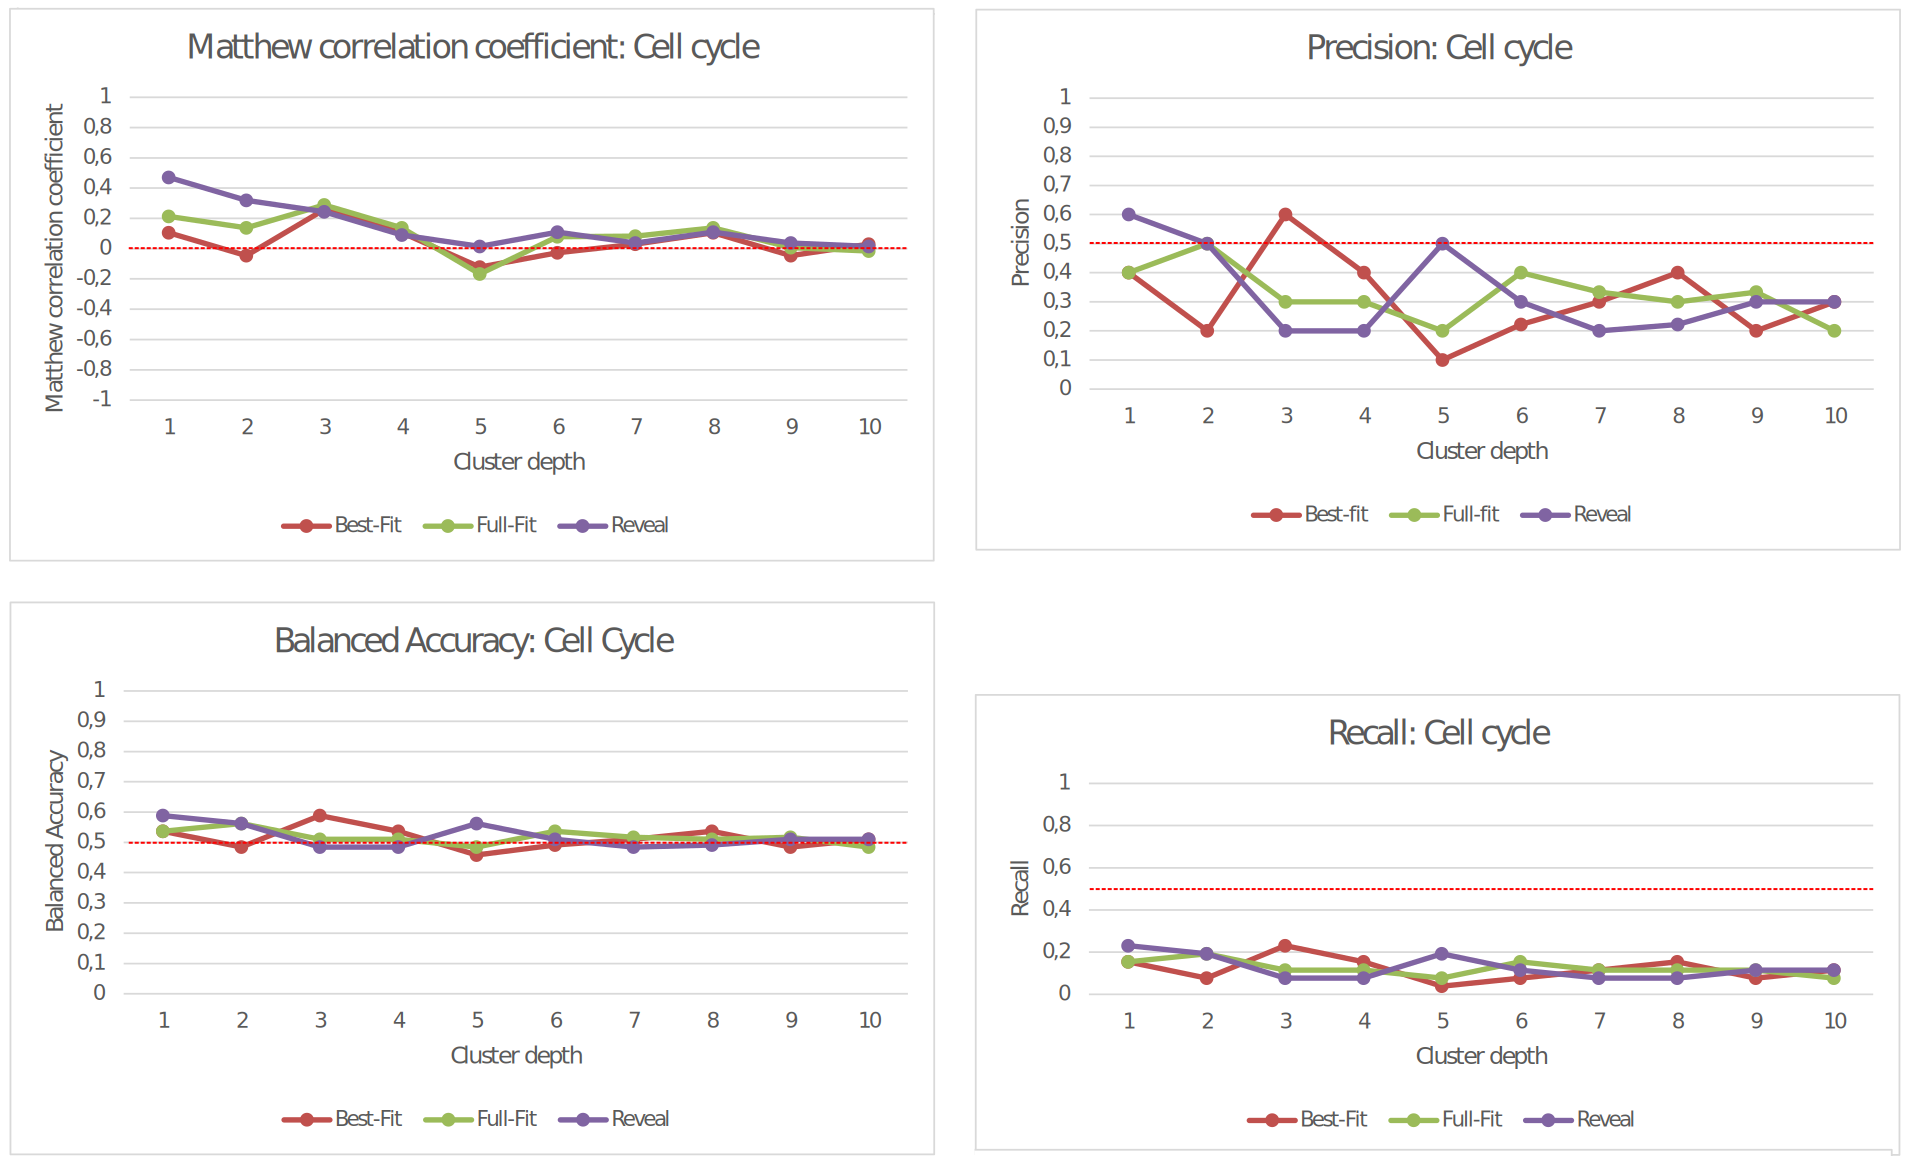
\includegraphics[width=1.0\textwidth]{./Bilder/Scoring/insilico/3_cellcycle_clusterdepth/insilico3.pdf}
\caption[Performance considering cluster depth \textit{d}]{Performance considering cluster depth \textit{d}}
\label{fig:7}
\end{figure}

\section{Pipeline of the Dream8 Challenge data set}
\begin{figure}[H]
\centering\includegraphics[width=0.6\textwidth]{./Bilder/pipeline_dream8.pdf}
\caption[pipelineDream8]{\textbf{Pipeline Dream8 Challenge. }}
\label{fig:9}
\end{figure}

%Raw structure
%-Pipeline fast identisch in silico pipeline mit einzigen Unterschied: input datensatz, km3+bestfit und gold standard selection.

%Learn-method: BESTFIT wird benutzt, weil: aus in silico weiß man, dass es mit fullfit gleich auf ist und durch das TS2B Paper, dass es die beste performance hat. 
% Prediction is converted to .bnet format for .sif format
%Goldstandard: welchen goldstandard hat die challenge verwendet und welchen gold standard benutze ich?
% Scoring gegen Prior aggregated network, aggregated network und letzten aus dem leaderboard(soll zeigen, dass Daten unbalanced sind), Erklären, warum ich mein eigenes Scoring mache und nicht dreamtools verwenden kann.
%Threshold: Wenn ich mehrere solutions habe, dann edge score berechenen über die Häufigeit von auftretenden Kanten, dann threshold verschieben, sodass von wenig bis viele tp sich ergeben = AUROC / = AUPR (Wegen runtime nicht gemacht,aber ich dann es ja für nur 3 runs zeigen?)


%Create 32 data set from training data -> txt. file
This section describes settings in the Dream8 Challenge pipeline which differ from the settings of the \textit{in silico} pipeline. 
The 'main' training data set of the Dream8 Challenge is converted into a \textit{txt} file format (Figure 2.8, Figure 3.1) by splitting each data set of a cell line into eight text files depending on the stimulus. Each of the resulting 32 text files contain about $\sim $85 sample points and about $\sim $45 antibody names (Figure 3.8).\\

\subsection*{Network inference}
%Quelle: TS2B Paper mit KM3 Empfehlung
%The python implementation of the inference algorithms is validated, such that a network up to 50 nodes can be inferred and the 
%Network inference: KM3+Best-Fit
The higher the \textit{in-degree} of the nodes and the amount of nodes in a network the higher is the complexity in a system and the higher is the computational cost of an inference algorithm. Due to computational limitations and a technical settings of 8 RAM and a Core i5 processor the application of Reveal to the Dream8 Challenge data set is an infeasible task (Figure 2.3). 
Furthermore, results of the \textit{in silico} data set show that the choice of abundance of sample points (Figure 3.6) and cluster depth (Figure 3.7) has no significant influence on the performance. An increasing \textit{in-degree} (Figure 3.4) shows an decreasing performance for all three algorithms, such that no algorithm can be excluded by this investigation. Thus, results of (Paper Quelle) regarding error assessment are taken into account, such that a recommanded combination of Best-Fit with the iterative \textit{k-means} algorithm with $d=3$ is applied to the Dream8 Challenge data set. This combination yielded the best performance, especially in complex systems.\\
%Tabelle in das supplementary,wo gezeigt wird wie gut die performance ist?
Predicted Boolean networks (\textit{bnet}) are converted into an Interaction graph (\textit{sif}) (Figure 4.2) and scored against a gold standard (Aggregated Network, Prior Aggregated Network). 
%Paper:TS2B Paper 
%Mit Fullfit auch das Scoring machen.

\subsection*{Gold standard selection in the Dream8 Challenge}
%Wie wird in der challenge gescored und (testdatensatz und AUROC AUPR, und wie score ich: Aggregated Network, Prior Aggregated Network, kein kantengewicht, kein threshold, daher Recall, Precision,....)
Since gold standard networks are often based on literature, learning novel connections in a network is restricted. Therefore the Dream8 Challenge did not provide a gold standard to the participants. Thus, a provided test data set was used as an abstracted representation of a gold standard to asses the algorithms performance by error assessment resulting in prior knowledge independent networks created with the training data set of the experimental data. It is useful to include prior knowledge, but this can come along with limitations, because it is difficult to truly mimic specific bilogical systems of interest.\\
%Quelle: Dream8 CHallenge Paper 
Additionally an \textit{in silico} data set covering main characteristics of the experimental setting, but without batch effects, is provided by the challenge. This \textit{in silico} data set is a tool for assessing the performance of an algorithm in an idealized setting. Hence, the performance of an algorithm excluding pertubational effects can be assessed.
The \textit{in silico} data set is generated from a nonlinear ordinary differential equations (ODE) model of the ERBB signaling pathway (ERBB:family of proteins containing four receptor tyrosine kinases, structually related to the epidermal grwoth factor receptor (EGFR)). Nevertheless pre-existing biological knowledge was included by several participants and seemed to be broadly benefical.\\
%Warum beneficial? Zeigen, dass die performance der gruppen mit prior knowledge nicht signifikant schlechter war als bei gruppen ohne

\subsection*{Evaluation in the Dream8 Challenge}
Due to different strategies of evaluating predictions, e.g. choice of the scoring metric and implementation approach, it is hard to compare the resulting performance between the participants. For this reason the Dream8 Challenge provides a standard scoring tool 'DREAMTools' python package.
%Quelle:  \citep{Cokelaer T, Bansal M, Bare C et al. DREAMTools: a Python package for scoring collaborative challenges [version 2; referees: 1 approved, 2 approved with reservations]. F1000Research 2016, 4:1030 (doi: 10.12688/f1000research.7118.2)}
This tool needs as input a \textit{sif} and an \textit{eda} file, where eda (electronic design automation) contains the confidence scores of edges in an Interaction Graph.\\
%Wurde erklärt, was ein confidence score ist?
DREAMtools compares the confidence scores \textit{eda} file of the prediction against the \textit{eda} file of a gold standard by classifying the data by a threshold $\tau$. Confidence scores below this threshold take a value of $0$ indicating an edge is less likely to occur and a confidence score above $\tau$ is taking a value of $1$ indicating an edge is potential. By increasing the threshold $\tau\in[0,1]$ the amount false positve decrases and false negative increase. 
Resulting calasses are put into a context of True Positve Rate ($TPR=\frac{TP}{TP+FN}$) and False Negative Rate ($FPR=\frac{FP}{FP+TN}$). This yields a set of values returning a value of the area under the receiver operating characteristic curve (AUROC).\\\\   
Similar to balanced accuracy the AUPR (area under the precision recall curve) metric is used for imbalanced classes in the confusion matrix taking precision and recall in relationship by shifting $\tau$.
%Verweis auf Anhang: Erklärung/Definition von AUPR und AUROC
%Bild einfügen von AUROC und AUPR

\subsection*{Gold standard selection for the Prediction (Best-Fit)}
This work makes use of an aggregated network for all 32 contexts and an aggregated prior network as a gold standard. These networks were submitted after finishing the challenge in 2016. The aggregated network is a compendium of 66 submissions of the participants with the best performance reduced by correlated submissions. The aggregated prior network is a combination of 10 prior knowledge networks that participants used as part of their submission (Table 3.2).
%Paper: Dream8 Challenge über aggregated networks
Predictions of all 74 participants of the Dream8 Challenge leaderboard  and the prediction in this thesis by Best-Fit are scored against the aggregated network and against the aggregated prior network, such that a new ranking reveals how Best-fit performs in relation to the participants' submission.

\begin{table}[H]
%\resizebox{\textwidth}{!}{
%{\tabcolsep=6pt%
\begin{center}
%\captionsetup{width=0.87\linewidth}
%\small
\begin{tabular}{l|l|l}
\toprule 
Network & $\# $ Edges & $\# $ Networks\\
 \hline\hline
Prediction (Best-Fit) & $\sim 140$ & 1\\
\rowcolor{black!10} Aggregated Network & $\sim 2200 $ & 66\\
Aggregated Prior Network & $\sim 1400$ & 10\\
\bottomrule
\end{tabular}
\captionof{table}{Network structure}
\end{center}
%}
\end{table} 

\subsection*{Evaluation for the Prediction (Best-Fit)}
In contrast to the Dream8 Challenge the networks are scored by scoring metrics of recall, precision, accuracy, balanced accuracy and matthew correlation coefficient. This is done, because computing the confidence score is computationally limited, thus DREAMtools could not be applied. 
For calculating the edge scores the pipeline has to run approximately a 100 times for obtaining a set of predictions, then counting the occurences of each edge in each prediction which would return a probability for each edge. One execution of the pipeline needs about 5 hours. Of course it was taken into account to use a cluster (e.g. Allegro), due to a lack of globally implemented bioconda for installing Pycluster, this approach failed. 


\newpage
\section{Results of the Dream8 Challenge data set}
\subsection*{Prediction versus Aggregated Network and Aggregated Prior Network}
Scoring the prediction of the inference algorithm Best-Fit against the aggregated network and the aggregated prior network (Figure 3.9) shows that there is an imbalance in the classes. Especially regarding the accuracy of $\sim 15\% $ when the prediction is scored against the aggregated network. Taking the balanced accuracy improves the performane of up to $\sim 40 \% $. The amount of edges differ in both networks a lot, such that the number of false negatives is tremendously high (Figure 3.2). The same imbalance is observed scoring the prediction against the aggregated prior network. Less edges of the aggregated prior network lead to a smaller improvement of the scoring values.\\
For emphasizing this observation the preiction is scored in Figure 3.10 instead against the aggregated prior network against a submission of the last participant (rank: 74.) of the Dream8 Challenge leaderboard.\\
For further analysis the accuracy is neglected, due to the imbalanced classes accuracy falsifies interpretation.
% High amount of FalseNegatives: Bad accuracy for prediction against aggregated network
% High amount of TrueNegatives: Good accuracy for prediction against aggregated network
%= Yield: Balanced accuracy is at random.
%Vllt. noch prediction vs. prior knowledge network mit einfügen
\begin{figure}[H]
\captionsetup{width=0.8\linewidth}
\centering
\includegraphics[width=0.8\textwidth]{./Bilder/Scoring/dreamchallenge/1_Balanced_vs_Unbalanced/balanced1.pdf}
\caption[Imbalanced classes (1)]{Imbalanced classes (1). Accuracy and Balanced Accuracy for the prediction scored against the aggregated network and aggregated prior network.}
\label{fig:10}
\end{figure}
 

\begin{figure}[H]
\captionsetup{width=0.8\linewidth}
\centering
\includegraphics[width=0.8\textwidth]{./Bilder/Scoring/dreamchallenge/1_Balanced_vs_Unbalanced/balanced2.pdf}
\caption[Imbalanced classes (2)]{Imbalanced classes (2). Accuracy and Balanced Accuracy for the prediction scored against the aggregated network and aggregated prior network.}
\label{fig:10}
\end{figure}

Figure 3.11 and Figure 3.12 show values of recall and precision for scoring the prediction against the aggregated network and the aggregated prior network. Recall ranges from $5,6\% $ to $7,7\% $ for the aggregated prior network and from $6,2\% $ to $7,5\% $ for the aggregated network. Both aggregated networks contain a lot more edges than the prediction, such that the number of true positive is much smaller than the number of false negatives. In contrast to precision, which is not taking false positives into account. \\\\

Hence, values for precision range for the aggregated network from $90,2\% $ to $97,8\% $ and for the aggregated prior network from $51,0\% $ to $66,6\% $. This is because the big size of the aggregated network covers most of the predicted edges, such that the number of false positives. This explaines why the precision of scoring against the aggregated prior network is worse. 

\begin{figure}[H]
\captionsetup{width=0.8\linewidth}
\centering
\includegraphics[width=0.8\textwidth]{./Bilder/Scoring/dreamchallenge/1_Balanced_vs_Unbalanced/balanced_rec_prec1.pdf}
\caption[Recall: Prediction versus Aggregated/Prior Network]{Recall: Prediction versus Aggregated/Prior Network}
\label{fig:10}
\end{figure}

\begin{figure}[H]
\captionsetup{width=0.8\linewidth}
\centering
\includegraphics[width=0.8\textwidth]{./Bilder/Scoring/dreamchallenge/1_Balanced_vs_Unbalanced/balanced_rec_prec2.pdf}
\caption[Precision: Prediction versus Aggregated/Prior Network]{Precision: Prediction versus Aggregated/Prior Network}
\label{fig:10}
\end{figure}
\newpage
\subsection*{New Ranking: Aggregated Network and Aggregated Prior Network}

In Figure 3.13-3.15 submitted networks of participants of the Dream8 Challenge are scored against the aggregated network and the aggregated prior network including the predicted network of Best-Fit. The networks are ranked by their value of balanced accuracy (BACC), Matthew correlation coefficient (MCC), precision and recall. This ranking results in a rank for the prediction depicted in Table 3.3 for each scoring case. It is noticed that scoring the prediction against the aggregated network yields a mean rank of $\sim 38$, which is much better than the mean rank of $\sim 45$ by scoring the prediction against the aggregated prior network. \\
%Wie kann das sein?

%Warum ist der MCC so viel besser als der BACC?
The Matthew correlation coefficient and the balanced accuracy are both used to assess the performance when the classes are imbalanced. But the MCC yields a better ranking for the prediction in both cases, the aggregated network and the aggregated prior network than the balanced accuracy. 



\begin{table}[H]
\begin{center}
%\captionsetup{width=0.87\linewidth}
%\scriptsize
\small
\begin{tabular}{l|c|c|c}
\toprule 
\textbf{Scoring metric} &\textbf{Type} & \textbf{Aggregated Network} & \textbf{Aggregated Prior Network}\\
 \hline\hline
MeanBACC & rank & 43 & 49\\
\rowcolor{black!10} MeanBACC & value & $\sim 0,0628$ &$\sim 0,4950$\\
MeanMCC & rank & 33 & 39\\
\rowcolor{black!10} MeanMCC & value &$ \sim 0,0097$ &$ \sim 0,0195$\\
MeanPrecision & rank & 33 & 45 \\
\rowcolor{black!10} MeanPrecision & value & $\sim 0,9436$& $\sim 0,5909$\\
MeanRecall & rank &42 & 47\\
\rowcolor{black!10} MeanRecall & value & $\sim0,0677$ & $\sim 0,0632$\\
\bottomrule
\end{tabular}
\captionof{table}{Ranking of the prediction}
\end{center}
%}
\end{table} 

% Precison and Recall
\begin{figure}[H]
\centering
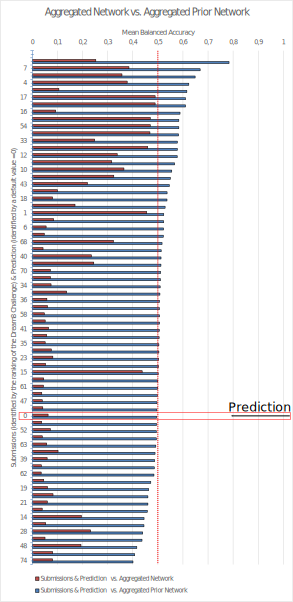
\includegraphics[width=0.62\textwidth]{./Bilder/Scoring/dreamchallenge/Meanbacc_vertical_comparison.pdf}
\caption[New Ranking Balanced Accuracy]{New Ranking (Balanced Accuracy): Aggr. Network and Aggr.Prior Network}
\label{fig:}
\end{figure}

\begin{figure}[H]
\centering
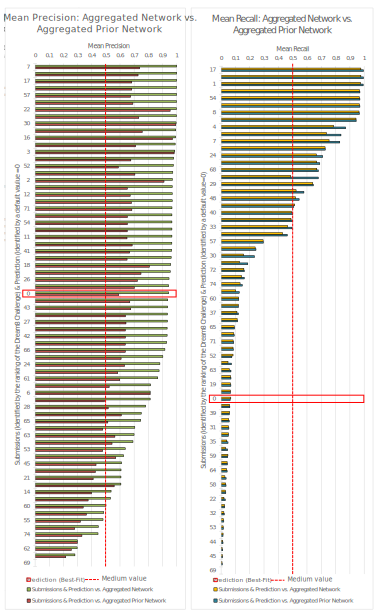
\includegraphics[width=0.82\textwidth]{./Bilder/Scoring/dreamchallenge/Recall_precision_vertical_comparison.pdf}
\caption[New Ranking: Precision and Recall]{New Ranking (Precision and Recall): Aggr. Network and Aggr.Prior Network}
\label{fig:}
\end{figure}

%MCC
\begin{figure}[H]
\centering
\includegraphics[width=0.6\textwidth]{./Bilder/Scoring/dreamchallenge/MeanMcc_vertical_comparison.pdf}
\caption[New Ranking: Matthew correlation coefficient]{New Ranking (Matthew correlation coefficient): Aggr. Network and Aggr.Prior Network}
\label{fig:}
\end{figure}




